% Options for packages loaded elsewhere
\PassOptionsToPackage{unicode}{hyperref}
\PassOptionsToPackage{hyphens}{url}
%
\documentclass[
  ignorenonframetext,
]{beamer}
\usepackage{pgfpages}
\setbeamertemplate{caption}[numbered]
\setbeamertemplate{caption label separator}{: }
\setbeamercolor{caption name}{fg=normal text.fg}
\beamertemplatenavigationsymbolsempty
% Prevent slide breaks in the middle of a paragraph
\widowpenalties 1 10000
\raggedbottom
\setbeamertemplate{part page}{
  \centering
  \begin{beamercolorbox}[sep=16pt,center]{part title}
    \usebeamerfont{part title}\insertpart\par
  \end{beamercolorbox}
}
\setbeamertemplate{section page}{
  \centering
  \begin{beamercolorbox}[sep=12pt,center]{part title}
    \usebeamerfont{section title}\insertsection\par
  \end{beamercolorbox}
}
\setbeamertemplate{subsection page}{
  \centering
  \begin{beamercolorbox}[sep=8pt,center]{part title}
    \usebeamerfont{subsection title}\insertsubsection\par
  \end{beamercolorbox}
}
\AtBeginPart{
  \frame{\partpage}
}
\AtBeginSection{
  \ifbibliography
  \else
    \frame{\sectionpage}
  \fi
}
\AtBeginSubsection{
  \frame{\subsectionpage}
}
\usepackage{amsmath,amssymb}
\usepackage{lmodern}
\usepackage{iftex}
\ifPDFTeX
  \usepackage[T1]{fontenc}
  \usepackage[utf8]{inputenc}
  \usepackage{textcomp} % provide euro and other symbols
\else % if luatex or xetex
  \usepackage{unicode-math}
  \defaultfontfeatures{Scale=MatchLowercase}
  \defaultfontfeatures[\rmfamily]{Ligatures=TeX,Scale=1}
\fi
% Use upquote if available, for straight quotes in verbatim environments
\IfFileExists{upquote.sty}{\usepackage{upquote}}{}
\IfFileExists{microtype.sty}{% use microtype if available
  \usepackage[]{microtype}
  \UseMicrotypeSet[protrusion]{basicmath} % disable protrusion for tt fonts
}{}
\makeatletter
\@ifundefined{KOMAClassName}{% if non-KOMA class
  \IfFileExists{parskip.sty}{%
    \usepackage{parskip}
  }{% else
    \setlength{\parindent}{0pt}
    \setlength{\parskip}{6pt plus 2pt minus 1pt}}
}{% if KOMA class
  \KOMAoptions{parskip=half}}
\makeatother
\usepackage{xcolor}
\newif\ifbibliography
\usepackage{graphicx}
\makeatletter
\def\maxwidth{\ifdim\Gin@nat@width>\linewidth\linewidth\else\Gin@nat@width\fi}
\def\maxheight{\ifdim\Gin@nat@height>\textheight\textheight\else\Gin@nat@height\fi}
\makeatother
% Scale images if necessary, so that they will not overflow the page
% margins by default, and it is still possible to overwrite the defaults
% using explicit options in \includegraphics[width, height, ...]{}
\setkeys{Gin}{width=\maxwidth,height=\maxheight,keepaspectratio}
% Set default figure placement to htbp
\makeatletter
\def\fps@figure{htbp}
\makeatother
\setlength{\emergencystretch}{3em} % prevent overfull lines
\providecommand{\tightlist}{%
  \setlength{\itemsep}{0pt}\setlength{\parskip}{0pt}}
\setcounter{secnumdepth}{-\maxdimen} % remove section numbering
\ifLuaTeX
\usepackage[bidi=basic]{babel}
\else
\usepackage[bidi=default]{babel}
\fi
\babelprovide[main,import]{spanish}
% get rid of language-specific shorthands (see #6817):
\let\LanguageShortHands\languageshorthands
\def\languageshorthands#1{}
\ifLuaTeX
  \usepackage{selnolig}  % disable illegal ligatures
\fi
\IfFileExists{bookmark.sty}{\usepackage{bookmark}}{\usepackage{hyperref}}
\IfFileExists{xurl.sty}{\usepackage{xurl}}{} % add URL line breaks if available
\urlstyle{same} % disable monospaced font for URLs
\hypersetup{
  pdftitle={Efecto traspaso del tipo de cambio a precios},
  pdfauthor={Jorge Orenos},
  pdflang={es-MX},
  hidelinks,
  pdfcreator={LaTeX via pandoc}}

\title{Efecto traspaso del tipo de cambio a precios}
\subtitle{Una estimación para Guatemala}
\author{Jorge Orenos}
\date{Agosto 2022}

\begin{document}
\frame{\titlepage}

\begin{frame}{Pregunta de investigación}
\protect\hypertarget{pregunta-de-investigaciuxf3n}{}
¿El efecto traspaso (pass-through) disminuye junto con la inflación?

\textbf{Objetivos}

\begin{itemize}
\tightlist
\item
  Comprobar si el pass-through disminuye en escenarios de inflación
  baja.
\item
  Verificar si la disminución del pass-through se debe al debilitamiento
  de la relación tipo de cambio y los precios.
\end{itemize}
\end{frame}

\begin{frame}{Introducción}
\protect\hypertarget{introducciuxf3n}{}
\begin{itemize}
\item
  En los últimos 30 años en Guatemala se ha hecho política monetaria
  bajo dos esquemas: Agregados Monetarios y el de Metas Explicitas de
  Inflación (EMEI).
\item
  Durante este periodo el Banco de Guatemala ha tenido éxito en
  controlar la inflación y anclar las expectativas de los agentes,
  especialmente en el EMEI.
\item
  Las series del tipo de cambio e inflación parecen exhibir un
  comportamiento indpendiente, pero se hace necesario comprobarlo y
  estimar el efecto del tipo de cambio sobre los precios en un periodo
  que incluya el EMEI.
\end{itemize}
\end{frame}

\begin{frame}{Comportamiento de la inflación en los últimos 30 años}
\protect\hypertarget{comportamiento-de-la-inflaciuxf3n-en-los-uxfaltimos-30-auxf1os}{}
\end{frame}

\begin{frame}{}
\protect\hypertarget{section}{}
\textbf{Comportamiento conjunto entre tipo de cambio e inflación}

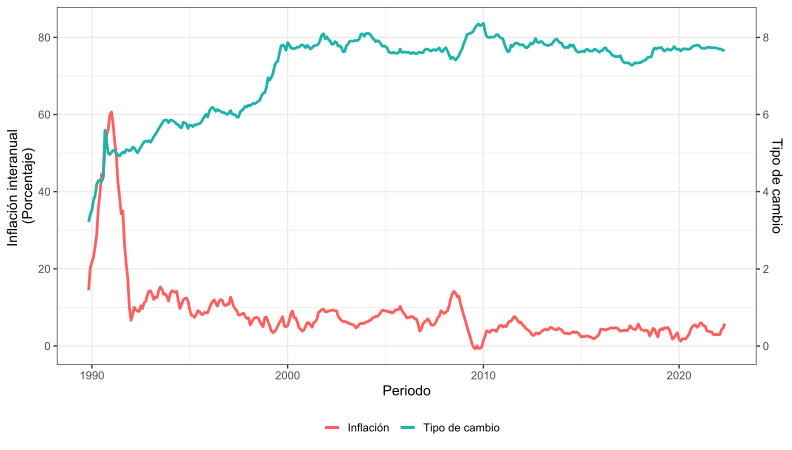
\includegraphics[width=8.33333in,height=\textheight]{D:/Documentos/PES/Para la tesis/Tesis/Pass through/Trabajo de graduación/Imagenes/Tipo de cambio e inflación.gif}
\end{frame}

\begin{frame}{Revisión literaria}
\protect\hypertarget{revisiuxf3n-literaria}{}
Efecto pass-through

\begin{itemize}
\tightlist
\item
  Definición del efecto pass-through (Goldberg y Knetter, 1996).
\item
  Reducción del pass-through ante el contexto inflacionario (John
  Taylor, 2000).
\item
  Modelo autorregresivo por umbrales.
\end{itemize}

\includegraphics[width=0.7\textwidth,height=\textheight]{D:/Documentos/PES/Para la tesis/Tesis/Pass through/Presentación/Imagenes presentación/TAR básico.png}

\begin{itemize}
\tightlist
\item
  Estudios México (Baqueiro, Díaz de León, \& Torres, 2004), Argentina
  (Brufman, Trajtenberg, \& Donaldson, 2016) y Guatemala (Eddy Carpiio,
  2008 y Banco de Guatemala, 2005).
\end{itemize}
\end{frame}

\begin{frame}{Metodología}
\protect\hypertarget{metodologuxeda}{}
\textbf{La especificación inicial del modelo fue:}

\includegraphics[width=0.85\textwidth,height=\textheight]{D:/Documentos/PES/Para la tesis/Tesis/Pass through/Presentación/Imagenes presentación/TAR general pass-through.png}

\includegraphics[width=0.65\textwidth,height=\textheight]{D:/Documentos/PES/Para la tesis/Tesis/Pass through/Presentación/Imagenes presentación/Variables TAR.png}

La variable que define el estado del sistema es el componente inercial
de la inflación
\end{frame}

\begin{frame}{}
\protect\hypertarget{section-1}{}
El modelo anterior se puede especificar en términos de una interacción
con una variable dummy

\includegraphics[width=1\textwidth,height=\textheight]{D:/Documentos/PES/Para la tesis/Tesis/Pass through/Presentación/Imagenes presentación/TAR general con dummy.png}

Donde

\includegraphics[width=1\textwidth,height=\textheight]{D:/Documentos/PES/Para la tesis/Tesis/Pass through/Presentación/Imagenes presentación/Primera dummy.png}

Las especificaciones anteriores cuentan con dos regímenes
inflacionarios:

si \(\Delta\%P_{t-1}<\tau\) régimen de inflación alta

si \(\Delta\%P_{t-1}\geq\tau\) régimen de inflación alta
\end{frame}

\begin{frame}{Datos utilizados}
\protect\hypertarget{datos-utilizados}{}
Todas las variables están en frecuencia mensual y abarcan el periodo
enero 2001 - mayo 2022.
\end{frame}

\end{document}
